Al comienzo de este trabajo nos propusimos generar un modelo de predicción de patogenicidad en polimorfismos de un sólo nucleótido (SNPs), tratando de mejorar y aumentar lo conseguido a partir del análisis del modelo realizado con las variables que nos aportó VarQ. Con el objetivo de responder la primera pregunta formulada inicialmente, buscamos trabajos de relevancia sobre el tema que nos permitiera incorporar una gran cantidad de variables nuevas, separadas en distintos grupos, según su interpretación biológica. Combinando estas variables con algoritmos de aprendizaje automático logramos una performance en la identificación de variantes patogénicas significativa, llegando a un AUC de 0.90 usando la totalidad de los SNPs reportados en Humsavar y a un AUC de 0.88 cuando evaluamos el modelo en el conjunto de variantes disponibles en el dataset de VarQ (ver figuras \ref{fig:curvas_auc_humsavar} y \ref{fig:curvas_auc_varq}).

El análisis estadístico de las variables de nuestro conjunto de datos nos permitió entender cómo el método estándar provisto en \texttt{scikit-learn} para calcular importancia de variables en métodos de ensamble se ve sesgado con la presencia de colinealidades en el conjunto de datos. En este sentido, el uso del método rfpimp [cita], como método alternativo de análisis de importancia de variables facilitó la interpretación biológica de los resultados obtenidos. . En particular, esto nos ayudó a responder nuestra segunda pregunta formulada en la introducción, al identificar variables de importancia en cada una de las dimensiones estudiadas. En el caso del modelo VarQ Curado, encontramos como variables relevantes a la variación de la energía (VARIATION\_ENERGY) y a la superficie accesible por parte del solvente (SASA). Luego, analizando las propiedades físico-químicas del cambio de aminoácido en la proteína, las variables más importantes fueron algunas de las matrices de sustitución (EX, PAM250, BLOSUM, etc.), aunque con un grado muy alto de correlación entre ellas, la diferencia en la aromaticidad (AROMATICITY\_DIFF) y la diferencia de hidrofobicidad (HYDROPHOBICITY) en la sustitución. Por último, en el caso genómico encontramos las variables con AUC univariado más elevado del trabajo, ambas referidas a la conservación filogenética del lugar (o el entorno) donde se produjo la variante: PHYLOP46WAY y PHASTCONS46WAY. Si bien el dataset de VarQ ya poseía una variable de conservación (CONS), ésta presentó un bajo nivel de relevancia en los modelos generados, el cual conjeturamos que se debe al origen de cálculo de esta variable: la misma se calcula a nivel de dominios funcionales Pfam, y con una familia mucho mayor de especies involucrado, sumado a su muy baja cobertura en los datasets estudiados.

Este trabajo también consistió en una comparación de distintos métodos de aprendizaje automático, buscando responder nuestro último interrogante. En la primera sección del desarrollo comparamos tres métodos clásicos con el dataset VarQ Curado: Regresión Logística, Support Vector Classifier y Random Forest, obteniendo mejores resultados con éste último. Luego en la última sección del trabajo comparamos Random Forest con un método de \textit{boosting}, XGBoost, en los datasets Integral y VarQ+Integral, mejorando la performance del modelo de un AUC de 0.88 a 0.90 y de 0.86 a 0.88 respectivamente, diferencias que mostraron ser estadísticamente significativas por el test de DeLong \cite{DeLong}. Si bien el tiempo de entrenamiento de los algoritmos fue relativamente bajo, esto se debe en parte  a haber acotado al subconjunto de hiperparámetros evaluados, por lo que hipotetizamos que todavía no se ha alcanzado el máximo nivel de desempeño posible de nuestro modelo.  

Por último, cabe recalcar que uno de los principales productos del esfuerzo realizado en este trabajo es la integración de un nuevo dataset que contiene numerosas variables estructurales y físico-químicos de la proteína, sumados a variables de tipo genómico que servirán como punto de partida para trabajos futuros del grupo. La combinación de estas variables demostró no ser superflua, mostrando una clara diferencia de performance entre el modelo Genómico (el de mejor desempeño independiente) y el Integral que contiene la sinergia de las distintas clases de variables exploradas.

\section{Trabajo Futuro}

Una de las principales tareas que quedaron pendientes en este trabajo fue el cálculo de variables de VarQ para las variantes de Humsavar. Al mismo tiempo la intersección del dataset Integral con VarQ dió como resultado una cobertura baja de las variables de conservación genómicas, por lo que también es necesario calcular estas variables para todas las variantes. 

Otro punto importante, como mencionamos en las conclusiones, es el espacio de búsqueda así como la técnica selección de hiperparámetros para mejorar el desempeño de  los algoritmos usados. Una las tareas posibles en este sentido es la implementación de un método más efectivo en la búsqueda de hiperparámetros óptimos, por ejemplo usando técnicas de optimización bayesiana. Por otro lado, la metodología de imputación de nulos en variables categóricas también admite el uso de enfoques más avanzados al utilizado en este trabajo. Otra posible dirección de exploración es la incorporación  de otros algoritmos de aprendizaje automático, como por ejemplo el uso de redes neuronales o métodos bayesianos de inferencia. 

Además de las mejoras posibles al modelo en términos de desempeño (AUC), creemos que hay puntos metodológicos que pueden ser modificados y mejorados. El trabajo no presenta una descripción estadística referida a la cantidad de variantes por proteína, por lo tanto no sabemos si tenemos algún sesgo al entrenar y evaluar con variantes ocurridas en la misma proteína. Esto incurriría en un tipo de razonamiento circular de tipo 2 según el trabajo de Grimm et al. (2015) \cite{doi:10.1002/humu.22768}.  

Los datasets utilizados poseen información adicional que no fue utilizada en nuestro trabajo, por ejemplo la enfermedad asociada a la variante. Utilizando esta información es posible restringirse a algún tipo de enfermedad particular, o reconocer clases de enfermedades, pasando de un problema de clasificación binario a uno de múltiples clases. 

\newpage


\begin{figure}[H]
\centering
\begin{subfigure}[b]{0.6\textwidth}
    \centering
    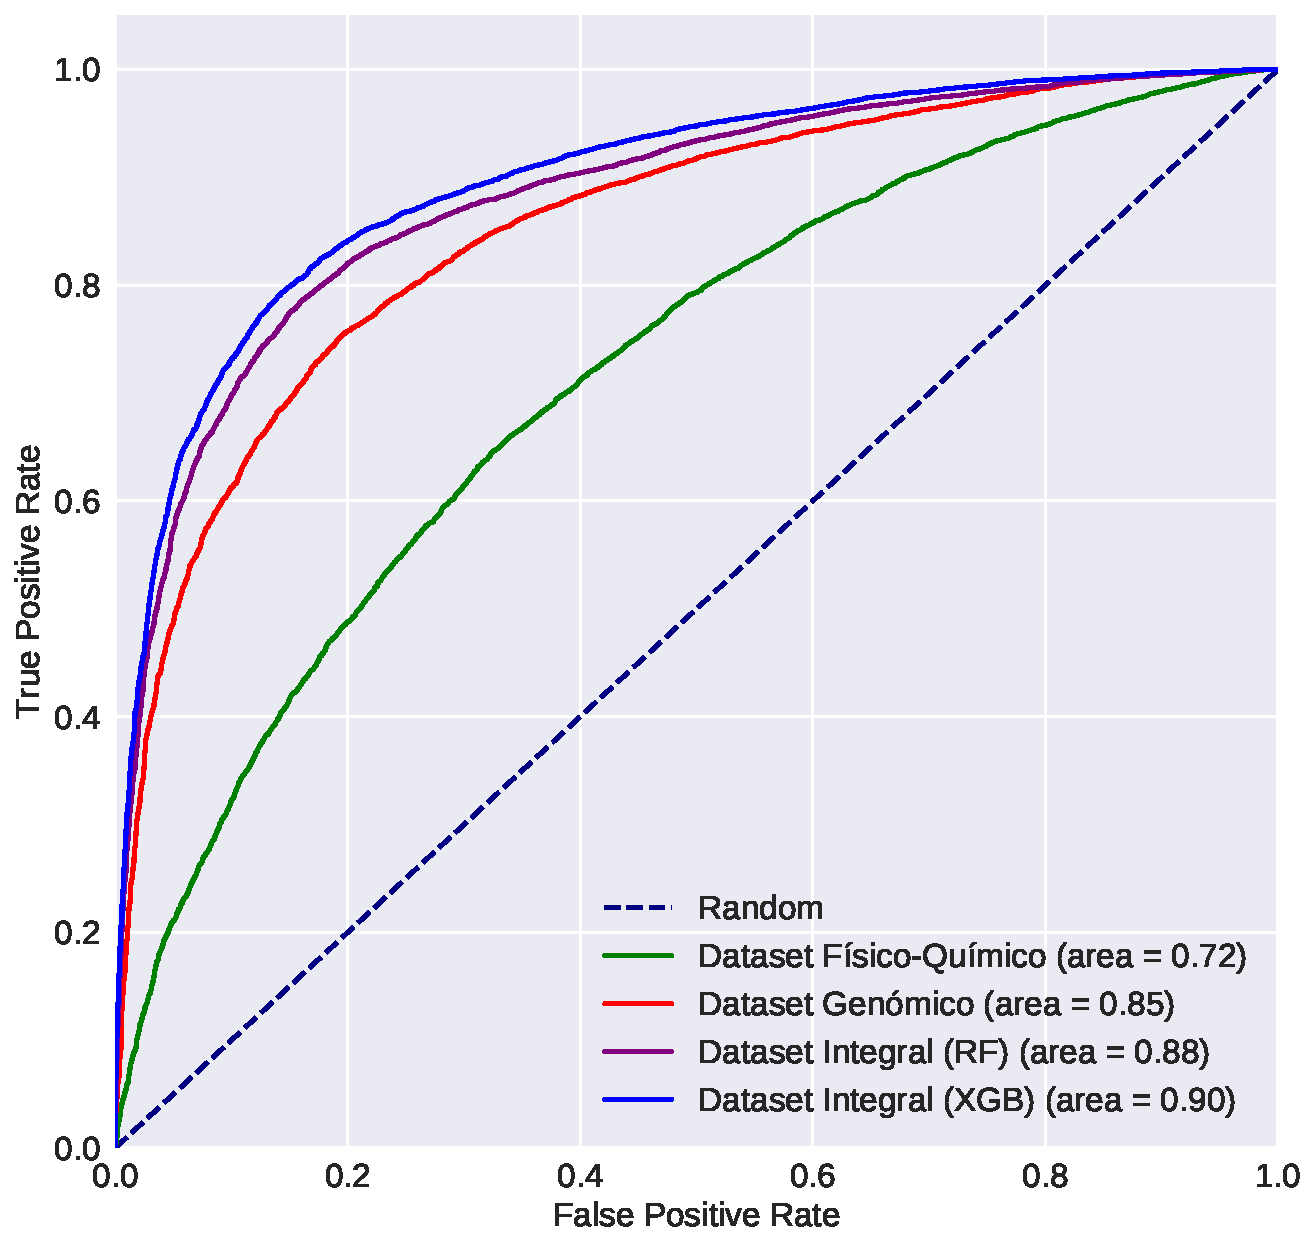
\includegraphics[width=\textwidth]{documents/latex/figures/4/curvas_auc_humsavar.pdf}
    \caption{Comparación de curvas ROC entre los datasets Físico-Químico, Genómico e Integral.}
    \label{fig:curvas_auc_humsavar}
\end{subfigure}

\hfill
\hfill

\begin{subfigure}[b]{0.6\textwidth}
    \centering
    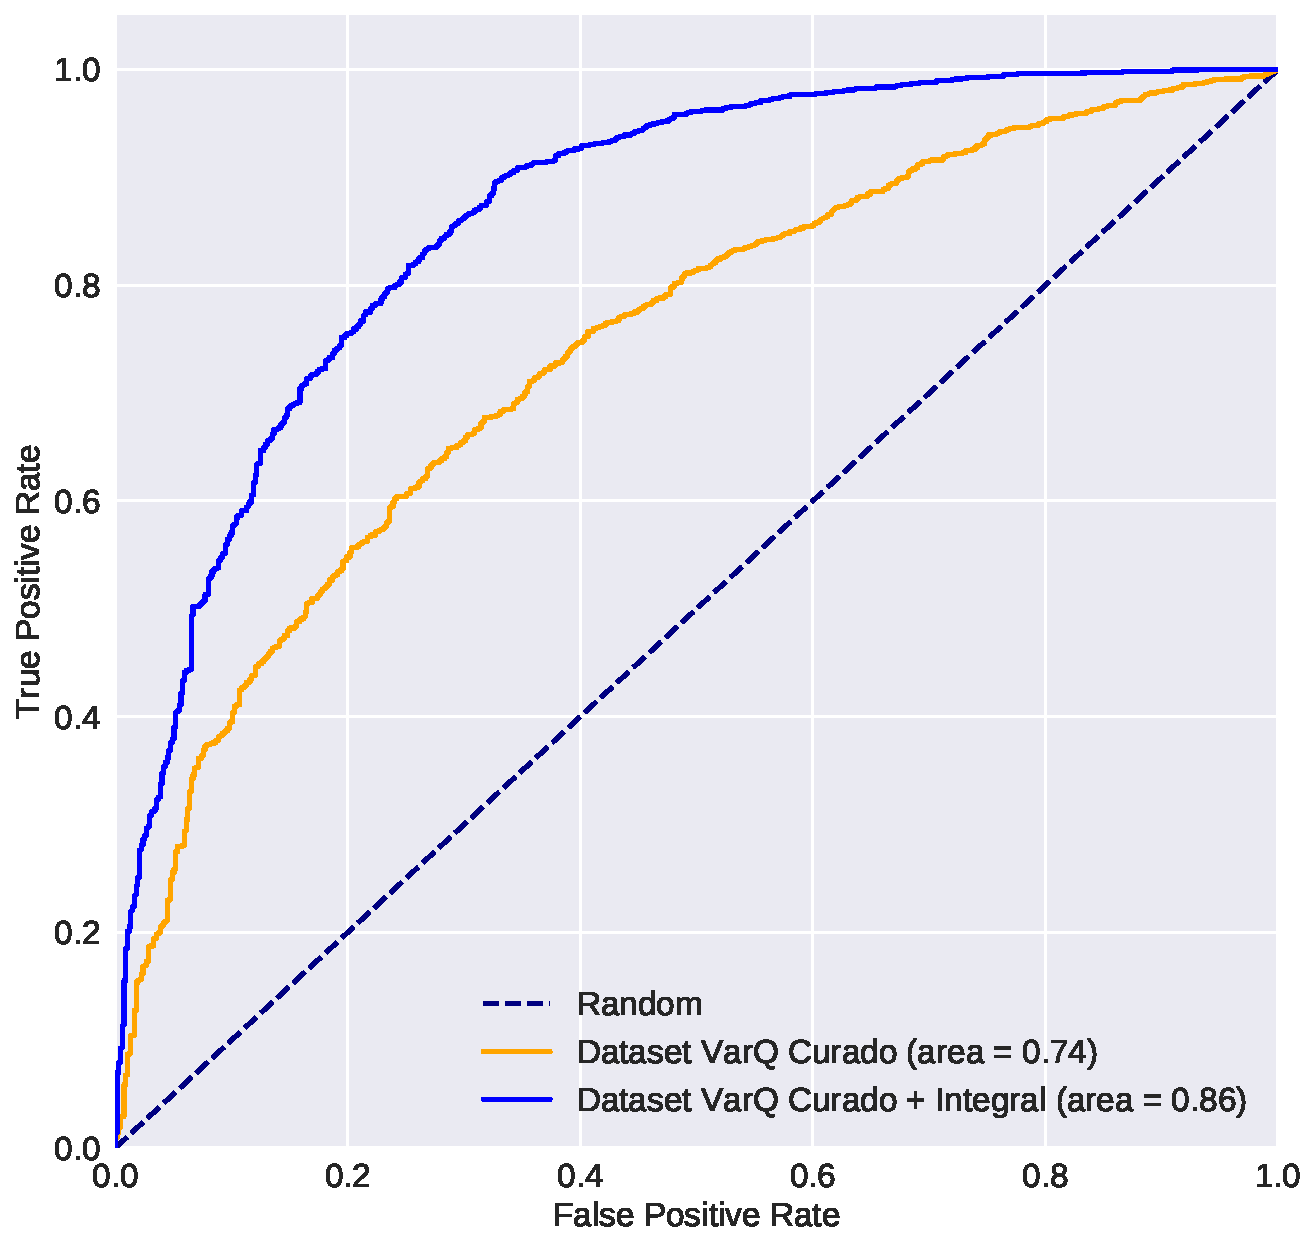
\includegraphics[width=\textwidth]{documents/latex/figures/4/curvas_auc_varq.pdf}
    \caption{Comparación de curvas ROC entre los datasets VarQ Curado y VarQ Curado + Integral.}
    \label{fig:curvas_auc_varq}
\end{subfigure}

\caption{Comparación de curvas AUC usando datasets con variantes de Humsavar y VarQ Curado.}
\end{figure}






